% 建议使用 XeLaTeX 或 LuaLaTeX 编译(中文与公式支持更佳)
\documentclass[UTF8,zihao=-4]{ctexart}

\usepackage[a4paper,margin=2.5cm]{geometry}
\usepackage{amsmath, amssymb, amsthm}
\usepackage{bm}
\usepackage{hyperref}
\usepackage{graphicx}
\usepackage{caption}
\usepackage{listings}
\usepackage{xcolor}
\usepackage{float}
\usepackage{placeins}
\graphicspath{{figures/}}

\lstdefinestyle{code}{
  basicstyle=\ttfamily\small,
  numbers=left,
  numberstyle=\tiny,
  numbersep=8pt,
  keywordstyle=\color{blue},
  commentstyle=\color{teal!70!black},
  stringstyle=\color{orange!70!black},
  showstringspaces=false,
  breaklines=true,
  frame=single,
  framerule=0.3pt,
  rulecolor=\color{black!15}
}
\lstset{style=code}

\title{Apriori 关联规则:原理、公式、应用与实战}
\author{}
\date{\today}

\begin{document}
\maketitle

\section{引言}
Apriori 算法利用“向下封闭性”在事务数据库中逐层挖掘频繁项集与关联规则。它在搜索过程中不断剪枝,将候选空间缩小至可能的频繁项集,并最终给出按支持度(support)、置信度(confidence)与提升度(lift)排序的规则,常用于市场篮分析、推荐等场景。

\section{原理与公式}
\subsection{支持度、置信度与提升度}
设项集 \(X\) 的支持度为
\begin{equation}
\operatorname{supp}(X) = \frac{\left|\{ T \mid X \subseteq T,\; T \in \mathcal{D}\}\right|}{|\mathcal{D}|}.
\end{equation}
对于规则 \(X \Rightarrow Y\)(\(X \cap Y = \emptyset\)),置信度与提升度分别为
\begin{align}
\operatorname{conf}(X \Rightarrow Y) &= \frac{\operatorname{supp}(X \cup Y)}{\operatorname{supp}(X)},\\
\operatorname{lift}(X \Rightarrow Y) &= \frac{\operatorname{conf}(X \Rightarrow Y)}{\operatorname{supp}(Y)}.
\end{align}
若提升度大于 1,说明二者存在正向关联;小于 1 则意味着潜在的替代关系。

\subsection{Apriori 迭代流程}
Apriori 以层次化方式扩展候选项集:
\begin{enumerate}
  \item 生成候选 1-项集,并筛除支持度低于 \(\texttt{min\_supp}\) 的项。
  \item 在第 \(k\) 层,将频繁 \((k-1)\)-项集连接得到候选 \(k\)-项集。
  \item 若候选的任意 \((k-1)\)-子集不是频繁项,则按 Apriori 性质剪枝。
  \item 扫描数据库计算支持度,保留满足阈值的项集。
  \item 重复以上步骤直至无候选项集,再生成满足 \(\texttt{min\_conf}\) 的规则。
\end{enumerate}
数据库扫描次数等于最大频繁项集的维度;因此阈值选择与数据稀疏性对性能影响显著。

\subsection{评价指标}
除支持度与置信度外,还可使用确信度(conviction)、杠杆率(leverage)等指标衡量规则价值。确信度定义为
\begin{equation}
\operatorname{conv}(X \Rightarrow Y) = \frac{1 - \operatorname{supp}(Y)}{1 - \operatorname{conf}(X \Rightarrow Y)},
\end{equation}
能惩罚失败概率较大的规则。通过可视化指标分布,可辅助设定适宜的阈值。

\section{应用与技巧}
\begin{itemize}
  \item \textbf{市场篮分析}:找到经常同时购买的商品组合,支持促销、陈列策略。
  \item \textbf{推荐系统}:在协同过滤之上增加可解释的共购规则。
  \item \textbf{异常检测}:识别低频但高风险的商品组合或行为模式。
  \item \textbf{实用建议}:离散化连续特征,去除出现频率极高的常用项,多轮调整 \(\texttt{min\_supp}\)、\(\texttt{min\_conf}\),并结合留出集或专家验证结果。
\end{itemize}

\section{Python 实战}
脚本 \texttt{gen\_apriori\_figures.py} 构造模拟事务数据,采用简化版 Apriori 实现挖掘频繁项集,绘制支持度-置信度散点与提升度分布,帮助调参与结果诊断。
\begin{lstlisting}[language=Python,caption={脚本 gen_apriori_figures.py 片段}]
from itertools import combinations

rules = []
for itemset, support in frequent_itemsets.items():
    for split in range(1, len(itemset)):
        for lhs in combinations(itemset, split):
            rhs = tuple(sorted(set(itemset) - set(lhs)))
            conf = support / frequent_itemsets[lhs]
            lift = conf / frequent_itemsets[rhs]
            rules.append((lhs, rhs, support, conf, lift))
\end{lstlisting}

\section{实验结果}
\begin{figure}[H]
  \centering
  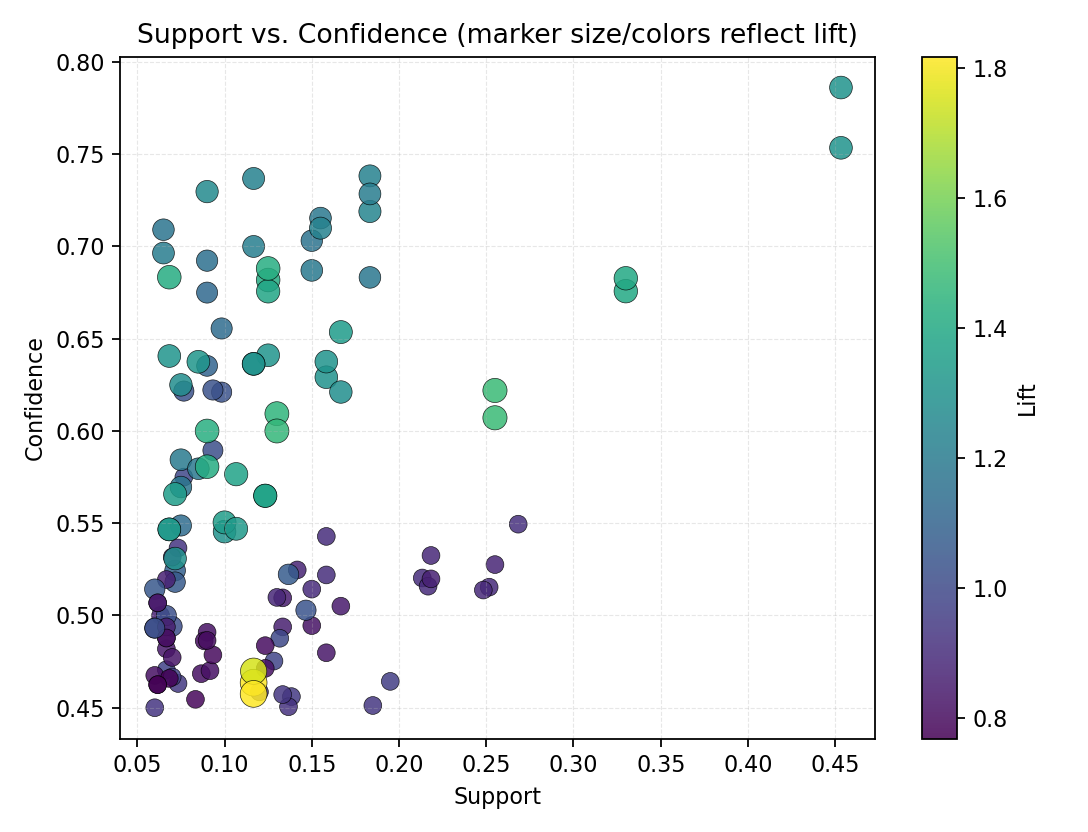
\includegraphics[width=0.82\linewidth]{apriori_support_confidence.png}
  \caption{关联规则的支持度-置信度散点图,点大小表示提升度}
  \label{fig:apriori_support_confidence_cn}
\end{figure}

\begin{figure}[H]
  \centering
  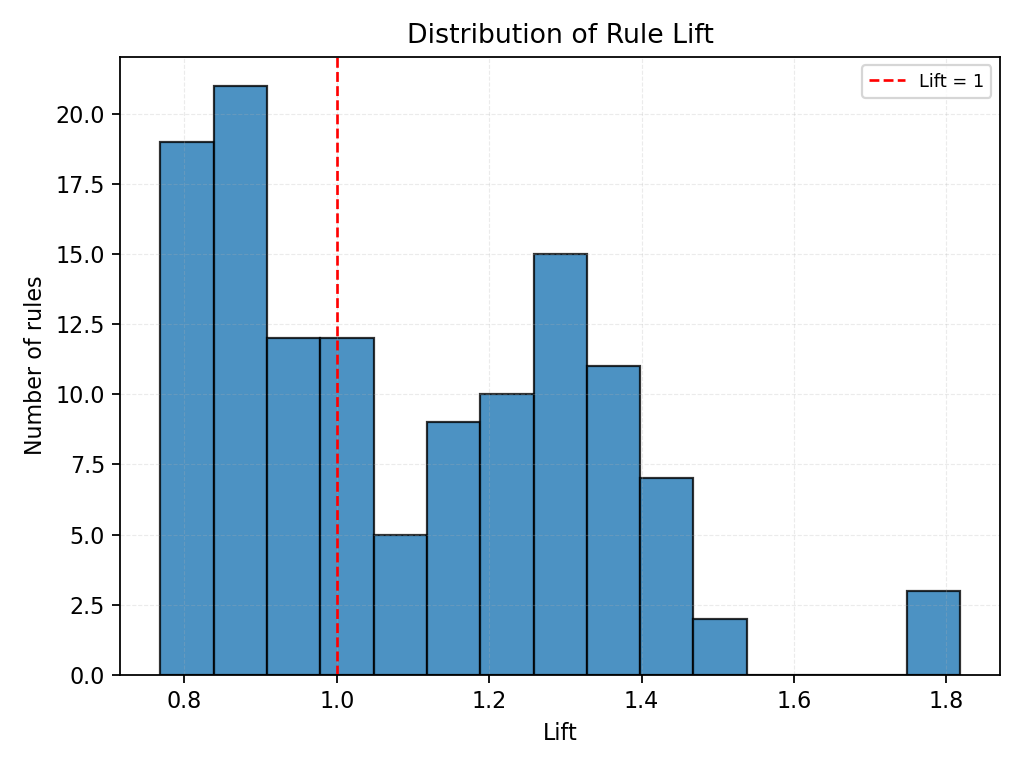
\includegraphics[width=0.78\linewidth]{apriori_lift_distribution.png}
  \caption{提升度分布,突出具有强关联性的规则}
  \label{fig:apriori_lift_distribution_cn}
\end{figure}

\FloatBarrier
\section{总结}
Apriori 遵循向下封闭性高效枚举频繁项集,生成可解释的关联规则。合理选择支持度、置信度与辅助指标,并结合领域知识进行验证,是成功应用的关键。示例展示了如何利用可视化把握调参尺度与规则质量。

\end{document}
